% THIS IS AN EXAMPLE DOCUMENT FOR VLDB 2012
% based on ACM SIGPROC-SP.TEX VERSION 2.7
% Modified by  Gerald Weber <gerald@cs.auckland.ac.nz>
% Removed the requirement to include *bbl file in here. (AhmetSacan, Sep2012)
% Fixed the equation on page 3 to prevent line overflow. (AhmetSacan, Sep2012)

\documentclass{vldb}
\usepackage{graphicx}
\usepackage{balance}  % for  \balance command ON LAST PAGE  (only there!)
\usepackage{todonotes}
\newcommand{\systemname}{\textbf{LOKI}\xspace}
\newcommand{\sysname}{\textbf{DOKI}\xspace}



% Include information below and uncomment for camera ready
\vldbTitle{Know Your Dataset}
\vldbAuthors{Poonam Kumari, supervised by Dr. Oliver Kennedy}
\vldbDOI{https://doi.org/TBD}

\begin{document}

% ****************** TITLE ****************************************

\title{Know Your Dataset}
%{A Sample {\ttlit Proceedings of the VLDB Endowment} Paper in LaTeX
%Format\titlenote{for use with vldb.cls}}


% possible, but not really needed or used for PVLDB:
%\subtitle{[Extended Abstract]
%\titlenote{A full version of this paper is available as\textit{Author's Guide to Preparing ACM SIG Proceedings Using \LaTeX$2_\epsilon$\ and BibTeX} at \texttt{www.acm.org/eaddress.htm}}}

% ****************** AUTHORS **************************************

% You need the command \numberofauthors to handle the 'placement
% and alignment' of the authors beneath the title.
%
% For aesthetic reasons, we recommend 'three authors at a time'
% i.e. three 'name/affiliation blocks' be placed beneath the title.
%
% NOTE: You are NOT restricted in how many 'rows' of
% "name/affiliations" may appear. We just ask that you restrict
% the number of 'columns' to three.
%
% Because of the available 'opening page real-estate'
% we ask you to refrain from putting more than six authors
% (two rows with three columns) beneath the article title.
% More than six makes the first-page appear very cluttered indeed.
%
% Use the \alignauthor commands to handle the names
% and affiliations for an 'aesthetic maximum' of six authors.
% Add names, affiliations, addresses for
% the seventh etc. author(s) as the argument for the
% \additionalauthors command.
% These 'additional authors' will be output/set for you
% without further effort on your part as the last section in
% the body of your article BEFORE References or any Appendices.

\numberofauthors{1} %  in this sample file, there are a *total*
% of EIGHT authors. SIX appear on the 'first-page' (for formatting
% reasons) and the remaining two appear in the \additionalauthors section.

\author{
% You can go ahead and credit any number of authors here,
% e.g. one 'row of three' or two rows (consisting of one row of three
% and a second row of one, two or three).
%
% The command \alignauthor (no curly braces needed) should
% precede each author name, affiliation/snail-mail address and
% e-mail address. Additionally, tag each line of
% affiliation/address with \affaddr, and tag the
% e-mail address with \email.
%
% 1st. author
\alignauthor
Poonam Kumari\\
       \affaddr{Supervised by Dr. Oliver Kennedy}\\
       \affaddr{State University of New York at Buffalo, Buffalo, NY, USA}\\
       \email{\{poonamku,okennedy\}@buffalo.edu}
}
% There's nothing stopping you putting the seventh, eighth, etc.
% author on the opening page (as the 'third row') but we ask,
% for aesthetic reasons that you place these 'additional authors'
% in the \additional authors block, viz.
\additionalauthors{Additional authors: John Smith (The Th{\o}rv\"{a}ld Group, {\texttt{jsmith@affiliation.org}}), Julius P.~Kumquat
(The \raggedright{Kumquat} Consortium, {\small \texttt{jpkumquat@consortium.net}}), and Ahmet Sacan (Drexel University, {\small \texttt{ahmetdevel@gmail.com}})}
\date{30 July 1999}
% Just remember to make sure that the TOTAL number of authors
% is the number that will appear on the first page PLUS the
% number that will appear in the \additionalauthors section.


\maketitle

\begin{abstract}
It has become very easy to obtain a large dataset for experimental analysis. Along with the ease arises the need to document the dataset for future use. Apart from documentation another challenge is posed by unlabeled or poorly labeled. Absence of labels, leads to difficulty in accessing the data.

We propose the design of a system, the first part of the system called LOKI would serve as a knowledge base for storing rules and column-naming heuristics, as well as provide an interactive tool: the LOKI editor for populating the knowledge-base. The second part of the system called DOKI would help start documentation for a dataset. 
\end{abstract}

\section{Motivation}
Big datasets are available in abundance and are being used by data scientists and database community for research purpose. These datasets are often curated, analyzed and forgotten without any documentation about the dataset itself. We propose to end this cycle by designing a system with a central goal of inferring column names by creating a knowledge base, which would store a collection of rules and column-naming heuristics (LOKI: Label Once and Keep It), as well as help start the documentation for a dataset.

So when presented a new dataset our system would start with creating labels using LOKI which would also help an analyst start documenting the dataset. Apart from creating a knowledge base LOKI provides an interactive tool for populating the knowledge base.\\
\\

\section{Research Questions}
Given a dataset the user wants to analyze, the system performs two steps (1) create labels (2) help start the documentation. Once a dataset is documented the analyst can save it for future use.  

LOKI helps in streamlining the process of developing schemas for unlabeled or poorly labeled datasets. It provides users with two modes of interaction: (1) A labeling interface that assists users in assigning names to existing columns of data, and (2) A discovery interface that helps users to search for columns representing particular concepts of interest. These interfaces are supported by a knowledge-base that combines expert-provided heuristics, learned characteristics, as well as historical feedback gathered from users about already-loaded datasets. Once the user has labeled or discovered a sufficient set of columns, LOKI generates appropriate data loading/initialization code (e.g., a CREATE TABLE or Spark DataFrame initializer).

Once a knowledge base is created, the next step is to start documenting the dataset. ~\ref{fig:DOKI} illustrates the different components of dataset that LOKI would store.

\begin{figure}[h]
	\centering
	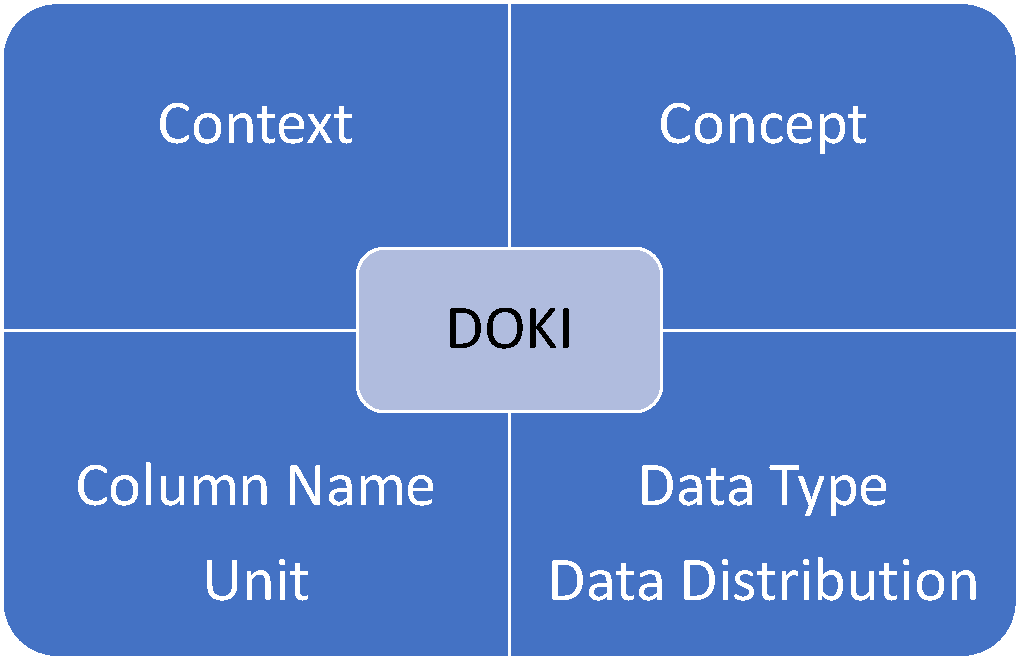
\includegraphics[width=0.8\columnwidth]{graphics/DOKI.pdf}
	\caption{Overview of Dataset Documentation}
	\label{fig:DOKI}
	\vspace*{-1mm}
\end{figure}

If a user points LOKI at a new dataset, LOKI proposes a schema for it. Input for a labeling query that helps infer column name for a new dataset is a set of columns and the knowledge base. The goal of the query is to identify a list of N distinct concepts, one for each attribute, that best fit the data in columns. For achieving this goal LOKI takes into account the context, concept, column name (if any), unit used in the column data, type of data present and data distribution of the column. 

\newtheorem{exmp}{Example}[section]
\begin{exmp}
	If LOKI is presented with~\ref{CropYields Dataset}, then the documentation would store details about columns and the dataset itself. For instance the values stored for column Fruithectares in~\ref{CropYields Dataset} would be context: agriculture, column name: Fruithectares, unit: Hectares, Data type: Float, Data distribution: Uniform.
\end{exmp}

Context stores the details of the domain to which the dataset belongs. Concepts correspond to names. Since the same name may be used in different contexts, multiple concepts can use the same column name. Similarly, a single concept may be associated with multiple names.
Unit refers to the mathematical unit associated with a column. e.g. Kilogram, Hectares, etc. Name stores the column name. Type of data present in the dataset whether it is numerical, categorical, datetime etc are stored as data type. Data distribution refers to the distribution that best describes a column. e.g Normal, uniform, zipfian etc.

\begin{table}
	\label{CropYields Dataset}
	\begin{center}
		\begin{tabular}{||c c c||} 
			\hline
			Fruithectares & Vegcount & Fruityieldtons \\ [0.5ex]
			\hline\hline
			5.8 & 0 & 1.5 \\ 
			\hline
			0 & 1.26 & 0 \\
			\hline
			2.6 & 0 & 7.2 \\
			\hline
			4.05 & 0.089 & 1.1 \\
			\hline
			0.17 & 6.5 & 0.48 \\ [1ex] 
			\hline
		\end{tabular}
	\end{center}
	\caption{CropYields Dataset}
\end{table}

Once LOKI starts documenting the dataset, analyst does not have to document it again, and is well versed with the dataset through information stored in knowledge base. The core component of LOKI is a knowledge-base that is used to identify column names. The knowledge-base is broken down into two parts, one heuristic-based, and the other feedback-based. In short, LOKI will allow users to assemble schemas on-demand, both (re-)discovering and incrementally refining schema definitions in response to changing data needs. 

\subsection{Challenges}
LOKI inferences column names 
\begin{enumerate}
	\item Column might match on multiple signatures
	\item Similar concepts with different signatures
	\item Similar signatures for different concepts
	\item Insufficient signal for signature based matching.
	->types of signature insufficient
	\item different signatures combine differently to id concepts
	\item performance
\end{enumerate}

\section{Related Work}
Other works have used data distribution for similar purposes. For example GestureQuery~\cite{nandi2013gestural} uses data similarity between two attributes to select candidate attributes for an equi-join.  

Wrangler \cite{kandel2011wrangler} and Potter's wheel \cite{raman2001potter} detect data domains through inclusion functions (e.g. regular expressions).
Wrangler in particular infers the data type of a column and highlights errors based on inconsistent data types. 
Wrangler also has several operators like split and unfold that create new columns.
The split operator decomposes composite data values into component distributions.  
The unfold operator reverses a table pivot, collapsing data laid out as key-value pairs into columns.  
A useful application of the LOKI knowledge-base that we hope to explore in future work is using it to detect opportunities for applying such operators.

An orthogonal approach to modeling and matching columns is to use ontologies, which express entities, facts, relations between facts and properties of relations
Ontologies like Yago \cite{fabian2007yago} could be used to identify semantic properties that relate columns.

A data summary called the data describer is used in \cite{ping2017datasynthesizer}. The data types, correlations and distributions of the attributes in a private dataset are listed. Each attribute is categorized into either numerical or non-numerical. If non-numerical attribute cannot be parsed as datetime then it is considered to be a string.

Data describer takes in a CSV file and infers the data types and domains. The attribute datatypes are parsed as numerical, datetime or string. We are inferring the datatypes as well. When run in correlated attribute mode, data describer provides corelation between attributes. We could use this functionality in LOKI.
% \todo{What exactly is the purpose of the data describer.  How is it used?  How do its goals differ from ours, and what are the implications on its design?} 

PADS \cite{fisher2005pads} helps users to understand the layout and meaning of data by designing syntactic descriptions of the data.
Based on the syntax, accumulators track the number of good values, the number of bad values, and the distribution of legal values.
This technique could be used in LOKI to help capture expert knowledge.

There is an increasing number of datasets in which well-structured attributes
(with or without a name) can be identified, each containing a set of values called a domain. There is lack of schema description in most of the datasets.
LSH Ensemble is used in \cite{zhu2016lsh} to find domains that maximally contain a query dataset, which can help to find datasets that best augment a given set of data.

\section{Research Plan}
We plan several extensions to LOKI focused on building and
refining a knowledge-base for storing column-naming heuristics.
• Use of contextual information: Contextual information
such as ontologies, units and data domains could be used to augment
the LOKI knowledge base (KB). We could use a network of
semantic relations such as BabelNet strengthen data models for
training the KB as well as providing curation recommendations
to experts. [2] • Recommendation of columns for query: Concepts
in the KB could be used to recommend columns that could be
in a query based on the columns that are already present. • Smarter
Matchers:We would develop matchers which regocognize a wider
spectrum of data. For example, regular expression matchers could
be used to detect geolocation data. Matchers which can identify
synonymous labels could help experts in the curation process.


\section{Conclusion}
This paper proposes the design of a system which would help build a knowledge base along with an interactive tool for populating the knowledge base. 


%\end{document}  % This is where a 'short' article might terminate

% ensure same length columns on last page (might need two sub-sequent latex runs)
\balance

%ACKNOWLEDGMENTS are optional
\section{Acknowledgments}
This work was supported by NSF Awards IIS-1750460, ACI-1640864
and by a gift from Oracle. The conclusions and opinions in this
work are solely those of the authors and do not represent the views
of the National Science Foundation or Oracle.


% The following two commands are all you need in the
% initial runs of your .tex file to
% produce the bibliography for the citations in your paper.
\bibliographystyle{abbrv}
\bibliography{vldb_sample}  % vldb_sample.bib is the name of the Bibliography in this case
% You must have a proper ".bib" file
%  and remember to run:
% latex bibtex latex latex
% to resolve all references

%APPENDIX is optional.
% ****************** APPENDIX **************************************
% Example of an appendix; typically would start on a new page
%pagebreak



\end{document}
